\documentclass[a4paper,11pt]{article}
\usepackage[utf8]{inputenc}
\usepackage[T1]{fontenc}
\usepackage{amsmath,amssymb}
\usepackage[a4paper,left=2cm,right=2cm,top=3.6cm,bottom=2.3cm,headheight=1.1cm,headsep=0.6cm,footskip=1cm]{geometry}
\usepackage{xcolor}
\usepackage{tikz}
\usetikzlibrary{calc,arrows.meta,positioning,shapes.geometric}
\usepackage{fancyhdr}
\usepackage{lastpage}
\usepackage{tabularx}
\usepackage{array}
\usepackage[most]{tcolorbox}
\usepackage{enumitem}
\usepackage{needspace}

% ---------- palet merah dan merah muda ----------
\definecolor{redx}{HTML}{B3202F}
\definecolor{pinkx}{HTML}{E0457B}
\definecolor{maroon}{HTML}{7A1C2C}
\definecolor{softbg}{HTML}{FDF1F4}
\definecolor{salmon}{HTML}{E8836F}
\newcommand{\dis}{\displaystyle}

\setlength{\parindent}{0pt}
\renewcommand{\arraystretch}{1.35}

\tikzset{
  ar/.style={-{Stealth[length=1.8mm]},thick,redx},
  box/.style={draw=redx,thick,rounded corners=3pt,fill=softbg,align=center,inner sep=4pt}
}

% ---------- header berwarna merah ----------
\pagestyle{fancy}
\fancyhf{}
\renewcommand{\headrulewidth}{0pt}
\fancyhead[L]{%
  \begin{tikzpicture}[remember picture,overlay]
    \fill[redx] ([yshift=-1.2cm]current page.north west) rectangle ([yshift=-3.15cm]current page.north east);
    \fill[pinkx] ([yshift=-3.15cm]current page.north west) rectangle ([yshift=-3.25cm]current page.north east);
  \end{tikzpicture}%
  \color{white}\bfseries\large Latihan Soal Polinomial}
\fancyhead[R]{\color{white}\small Diunduh dari website \textbf{Math1729}\ \,|\,\ 5 Oktober 2026}
\fancyfoot[L]{\small\color{redx}Math1729 --- Polinomial}
\fancyfoot[R]{\small\color{redx}Halaman \thepage\ dari \pageref{LastPage}}

% ---------- komponen ----------
\newcounter{no}
\newcommand{\bagian}[2]{\par\Needspace{6\baselineskip}\vspace{1.0em}\noindent
  \begin{tcolorbox}[colback=redx,colframe=redx,coltext=white,boxrule=0pt,arc=2pt,left=6pt,right=6pt,top=3pt,bottom=3pt]
  \textbf{#1}\hfill{\small #2}\end{tcolorbox}\setcounter{no}{0}\par\vspace{-0.3em}}
\newcommand{\tingkat}[2]{\par\Needspace{7\baselineskip}\vspace{0.6em}\noindent
  {\color{pinkx}\rule{3pt}{1.1em}}\ {\color{redx}\bfseries #1}\ {\small\color{gray}--- #2}\par\vspace{0.1em}}
\newcommand{\soal}[2]{\par\vspace{0.75em}\stepcounter{no}\noindent
  \begin{minipage}[t]{1.8em}\textbf{\theno.}\end{minipage}%
  \begin{minipage}[t]{\dimexpr\linewidth-1.8em\relax}#1\par\vspace{0.35em}#2\end{minipage}\par}
\newcommand{\poin}[1]{\hfill{\small\color{redx}[#1 poin]}}

% teks di kiri, gambar di kanan
\newcommand{\gbr}[2]{\noindent\begin{minipage}[t]{0.56\linewidth}#1\end{minipage}\hfill\raisebox{\ht\strutbox}{\begin{minipage}[t]{0.41\linewidth}\vspace{0pt}\centering#2\end{minipage}}}

% pilihan jawaban
\newcommand{\pil}[5]{\begin{tabularx}{\linewidth}{@{}*{5}{X}@{}}\textbf{A.}\;#1 & \textbf{B.}\;#2 & \textbf{C.}\;#3 & \textbf{D.}\;#4 & \textbf{E.}\;#5\end{tabularx}}
\newcommand{\pilx}[5]{\begin{tabularx}{\linewidth}{@{}*{3}{X}@{}}\textbf{A.}\;#1 & \textbf{B.}\;#2 & \textbf{C.}\;#3\\[10pt] \textbf{D.}\;#4 & \textbf{E.}\;#5 & \end{tabularx}}
\newcommand{\jwb}{\hfill Jawaban: \rule{4.5cm}{0.4pt}}

\begin{document}
\thispagestyle{fancy}

\begin{center}
  {\color{redx}\fontsize{22}{26}\selectfont\bfseries Latihan Soal Polinomial\par}
  \vspace{2pt}
  {\color{pinkx}\large Nilai, Kesamaan, Pembagian, Teorema Sisa dan Faktor, Akar-akar, serta Penalaran Polinomial\par}
\end{center}
\vspace{2pt}
\begin{tcolorbox}[colback=softbg,colframe=redx!40,boxrule=0.6pt,arc=3pt,left=8pt,right=8pt,top=5pt,bottom=5pt]
\noindent\textbf{Nama} : \rule{4.6cm}{0.4pt}\hfill\textbf{Kelas} : \rule{2.2cm}{0.4pt}\hfill\textbf{Skor} : \rule{2.2cm}{0.4pt}
\end{tcolorbox}
\vspace{2pt}
\begin{tcolorbox}[colback=white,colframe=pinkx,boxrule=0.8pt,arc=3pt,left=8pt,right=8pt,top=4pt,bottom=4pt,title={\bfseries Petunjuk Pengerjaan},coltitle=white,fonttitle=\small]
\small
\begin{enumerate}[leftmargin=1.4em,itemsep=1pt,topsep=1pt]
\item Soal terdiri atas \textbf{20 pilihan ganda} (5 mudah, 5 sedang, 5 sulit, 5 HOTS), \textbf{5 isian singkat}, dan \textbf{5 uraian (essay)}. Soal disusun berjenjang dari mudah sampai HOTS. Bentuk soal mengikuti pola tes penalaran terbaru (UTBK-SNBT): pilihan ganda lima opsi, pernyataan majemuk (benar/salah), isian singkat, soal berbasis grafik dan konteks, serta penalaran pembuktian. Alokasi waktu yang disarankan: 120 menit.
\item Skor: pilihan ganda 2 poin, isian singkat 4 poin, uraian 8 poin per soal (total 100 poin). Tidak ada pengurangan skor untuk jawaban salah.
\item Notasi: $P(x)$ adalah polinomial (suku banyak), \textit{habis dibagi} berarti sisa pembagiannya nol, dan $\deg P$ adalah derajat $P$. Semua koefisien dan akar adalah bilangan real kecuali disebutkan lain. Gambar tidak selalu digambar sesuai skala.
\item Bilangan desimal ditulis dengan tanda koma. Jawaban pecahan ditulis dalam bentuk paling sederhana.
\item Kalkulator tidak diperkenankan.
\end{enumerate}
\end{tcolorbox}

% =====================================================================
\bagian{A. Pilihan Ganda}{20 soal $\times$ 2 poin = 40 poin. Pilih satu jawaban yang paling tepat.}

\tingkat{Tingkat Mudah}{soal 1 sampai 5}
\soal{Perhatikan polinomial $P(x)=(2x-1)^3(x^2+1)(x-3)$. Jumlah derajat dan koefisien utama $P(x)$ adalah \dots.}{\pil{$8$}{$11$}{$14$}{$17$}{$20$}}
\soal{Diketahui $3x^2-5x+7\equiv a(x-1)^2+b(x-1)+c$ untuk setiap $x$. Nilai $a+b+c$ adalah \dots.}{\pil{$3$}{$5$}{$6$}{$7$}{$9$}}
\soal{Polinomial $P(x)=x^3+ax^2-5x+6$ dibagi $x-1$ bersisa $4$. Sisa pembagian $P(x)$ oleh $x+2$ adalah \dots.}{\pil{$12$}{$16$}{$20$}{$24$}{$32$}}
\soal{\gbr{Gambar menunjukkan grafik polinomial berderajat $3$ yang memotong sumbu-$x$ di $x=-2$, $x=1$, dan $x=3$, serta melalui titik $(0,12)$. Jika polinomial tersebut adalah $P(x)$, nilai $P(4)$ adalah \dots.}{%
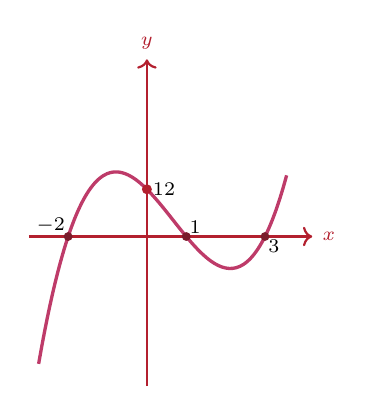
\begin{tikzpicture}[x=0.5cm,y=0.05cm]
\draw[->,thick,redx] (-3,0)--(4.2,0) node[right,font=\scriptsize]{$x$};
\draw[->,thick,redx] (0,-38)--(0,45) node[above,font=\scriptsize]{$y$};
\draw[pinkx!85!black,very thick] plot[domain=-2.75:3.55,samples=70,smooth] (\x,{2*(\x+2)*(\x-1)*(\x-3)});
\fill[maroon] (-2,0) circle (1.6pt) (1,0) circle (1.6pt) (3,0) circle (1.6pt);
\fill[redx] (0,12) circle (1.8pt);
\node[font=\scriptsize,above left,inner sep=1pt] at (-2,0) {$-2$};
\node[font=\scriptsize,above right,inner sep=1pt] at (1,0) {$1$};
\node[font=\scriptsize,below right,inner sep=1pt] at (3,0) {$3$};
\node[font=\scriptsize,right,inner sep=2pt] at (0,12) {$12$};
\end{tikzpicture}}}{\pil{$12$}{$18$}{$24$}{$36$}{$48$}}
\soal{Hasil bagi pembagian $2x^3-5x^2-4x+3$ oleh $2x-1$ adalah \dots.}{\pilx{$x^2-2x-3$}{$2x^2-4x-6$}{$x^2+2x-3$}{$2x^2+x-5$}{$x^2-2x+3$}}

\tingkat{Tingkat Sedang}{soal 6 sampai 10}
\soal{Polinomial $P(x)$ dibagi $x^2-4$ bersisa $3x+1$, dan dibagi $x-3$ bersisa $4$. Sisa pembagian $P(x)$ oleh $(x-2)(x-3)$ adalah \dots.}{\pilx{$3x+1$}{$-3x+1$}{$3x+13$}{$-3x+13$}{$-3x+7$}}
\soal{Diketahui $\alpha,\beta,\gamma$ adalah akar-akar polinomial $P(x)=x^3-3x^2-6x+8$. Perhatikan pernyataan berikut.
\begin{enumerate}[label=(\arabic*),leftmargin=1.8em,itemsep=0pt,topsep=2pt]
\item $x+2$ merupakan faktor dari $P(x)$.
\item $\alpha^2+\beta^2+\gamma^2=21$.
\item Sisa pembagian $P(x)$ oleh $x-2$ adalah $8$.
\item $\dis\frac1\alpha+\frac1\beta+\frac1\gamma=-\frac34$.
\end{enumerate}
Pernyataan yang benar adalah \dots.}{\begin{tabularx}{\linewidth}{@{}*{3}{X}@{}}\textbf{A.}\;(1) dan (2) saja & \textbf{B.}\;(1) dan (3) saja & \textbf{C.}\;(2) dan (4) saja\\[3pt] \textbf{D.}\;(1), (2), dan (4) saja & \textbf{E.}\;(1), (2), (3), dan (4) & \end{tabularx}}
\soal{Persamaan $2x^3-9x^2+7x+6=0$ mempunyai tiga akar real. Selisih akar terbesar dan akar terkecil adalah \dots.}{\pil{$\dis\frac12$}{$\dis\frac32$}{$\dis\frac52$}{$3$}{$\dis\frac72$}}
\soal{Polinomial $P(x)=x^4+ax^3-7x^2+bx+12$ habis dibagi $(x-1)(x+3)$. Nilai $a\cdot b$ adalah \dots.}{\pil{$-24$}{$-16$}{$-6$}{$10$}{$16$}}
\soal{\gbr{Selembar karton berbentuk persegi panjang berukuran $30$ cm $\times$ $18$ cm. Di keempat sudutnya dipotong persegi berukuran $x$ cm $\times$ $x$ cm (daerah arsiran), lalu sisanya dilipat menjadi kotak tanpa tutup. Jika volume kotak adalah $448$ cm$^3$, jumlah semua nilai $x$ yang mungkin adalah \dots.}{%
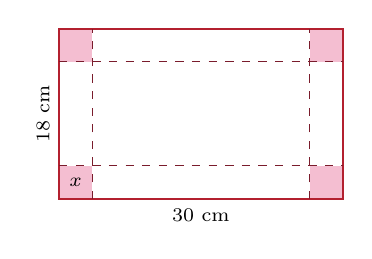
\begin{tikzpicture}
\def\W{3.6}\def\H{2.16}\def\c{0.42}
\fill[pinkx!35] (0,0) rectangle (\c,\c);
\fill[pinkx!35] ({\W-\c},0) rectangle (\W,\c);
\fill[pinkx!35] (0,{\H-\c}) rectangle (\c,\H);
\fill[pinkx!35] ({\W-\c},{\H-\c}) rectangle (\W,\H);
\draw[redx,thick] (0,0) rectangle (\W,\H);
\draw[maroon,dashed] (\c,0)--(\c,\H) ({\W-\c},0)--({\W-\c},\H) (0,\c)--(\W,\c) (0,{\H-\c})--(\W,{\H-\c});
\node[font=\scriptsize] at ({\c/2},{\c/2}) {$x$};
\node[font=\scriptsize,below] at ({\W/2},0) {$30$ cm};
\node[font=\scriptsize,rotate=90,above] at (0,{\H/2}) {$18$ cm};
\end{tikzpicture}}}{\pil{$1$}{$7$}{$8$}{$23$}{$24$}}

\tingkat{Tingkat Sulit}{soal 11 sampai 15, setara UTBK}
\soal{Sisa pembagian $x^{100}+2x^{50}+3$ oleh $x^2+x+1$ adalah \dots.}{\pil{$x+1$}{$-x+1$}{$-x-1$}{$x-1$}{$0$}}
\soal{\gbr{Gambar menunjukkan grafik polinomial $P(x)$ berderajat $4$ yang memotong sumbu-$x$ di $x=-2$ dan $x=3$, menyinggung sumbu-$x$ di $x=1$, serta melalui titik $(0,6)$. Sisa pembagian $P(x)$ oleh $(x-2)(x+1)$ adalah \dots.}{%
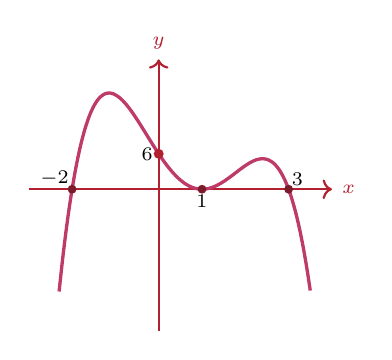
\begin{tikzpicture}[x=0.55cm,y=0.075cm]
\draw[->,thick,redx] (-3,0)--(4,0) node[right,font=\scriptsize]{$x$};
\draw[->,thick,redx] (0,-24)--(0,22) node[above,font=\scriptsize]{$y$};
\draw[pinkx!85!black,very thick] plot[domain=-2.3:3.5,samples=80,smooth] (\x,{-(\x+2)*(\x-1)^2*(\x-3)});
\fill[maroon] (-2,0) circle (1.6pt) (1,0) circle (1.6pt) (3,0) circle (1.6pt);
\fill[redx] (0,6) circle (1.8pt);
\node[font=\scriptsize,above left,inner sep=1pt] at (-2,0) {$-2$};
\node[font=\scriptsize,below,inner sep=2pt] at (1,0) {$1$};
\node[font=\scriptsize,above right,inner sep=1pt] at (3,0) {$3$};
\node[font=\scriptsize,left,inner sep=2pt] at (0,6) {$6$};
\end{tikzpicture}}}{\pil{$-4x+6$}{$4x-12$}{$-3x+12$}{$4x+12$}{$-4x+12$}}
\soal{Akar-akar persamaan $x^3-14x^2+kx-64=0$ membentuk barisan geometri. Nilai $k$ adalah \dots.}{\pil{$28$}{$42$}{$48$}{$56$}{$64$}}
\soal{Sisa pembagian $x^5-2x^3+7$ oleh $x^2-2x+1$ adalah \dots.}{\pil{$-x+7$}{$-x+6$}{$x+5$}{$2x+4$}{$6$}}
\soal{Banyak bilangan bulat $x$ yang memenuhi pertidaksamaan $x^4-2x^3-3x^2+4x+4\le0$ adalah \dots.}{\pil{$0$}{$1$}{$2$}{$3$}{$4$}}

\tingkat{Tingkat HOTS}{soal 16 sampai 20, penalaran tingkat tinggi gaya UTBK}
\soal{Polinomial $P(x)$ berderajat $4$ dengan koefisien $x^4$ sama dengan $1$ memenuhi $P(1)=10$, $P(2)=20$, dan $P(3)=30$. Nilai $P(0)+P(4)$ adalah \dots.}{\pil{$40$}{$50$}{$56$}{$60$}{$64$}}
\soal{Polinomial $P(x)$ memenuhi $P(x+1)-P(x)=6x^2+4x+1$ untuk setiap $x$, dan $P(0)=4$. Nilai $P(6)$ adalah \dots.}{\pil{$330$}{$396$}{$400$}{$404$}{$432$}}
\soal{Perhatikan empat pernyataan berikut tentang polinomial. Tentukan setiap pernyataan benar (B) atau salah (S).\par\smallskip
\begin{tabularx}{\linewidth}{@{}c X c c@{}}
\hline
\textbf{No.} & \textbf{Pernyataan} & \textbf{B} & \textbf{S}\\ \hline
(1) & Setiap polinomial berderajat $3$ dengan koefisien real memiliki paling sedikit satu akar real. & $\square$ & $\square$\\
(2) & Polinomial $x^4+4$ tidak dapat dinyatakan sebagai hasil kali dua polinomial berderajat $2$ dengan koefisien bulat. & $\square$ & $\square$\\
(3) & Jika $P(x)$ dibagi $x-1$ bersisa $2$ dan dibagi $x+1$ juga bersisa $2$, maka sisa pembagian $P(x)$ oleh $x^2-1$ adalah $2$. & $\square$ & $\square$\\
(4) & Jika $P(x)$ berkoefisien bulat, maka $P(7)-P(3)$ selalu habis dibagi $5$. & $\square$ & $\square$\\ \hline
\end{tabularx}\par\smallskip
Urutan nilai kebenaran pernyataan (1) sampai (4) yang tepat adalah \dots.}{\begin{tabularx}{\linewidth}{@{}*{3}{X}@{}}\textbf{A.}\;B, B, S, S & \textbf{B.}\;B, S, B, S & \textbf{C.}\;S, B, B, S\\[3pt] \textbf{D.}\;B, S, B, B & \textbf{E.}\;S, S, B, B & \end{tabularx}}
\soal{Misalkan $a,b,c$ adalah akar-akar persamaan $x^3-2x^2+3x-5=0$. Persamaan kubik yang akar-akarnya $a^2$, $b^2$, dan $c^2$ adalah \dots.}{\begin{tabularx}{\linewidth}{@{}lX@{}}
\textbf{A.} & $x^3+2x^2-11x-25=0$\\
\textbf{B.} & $x^3-2x^2-11x+25=0$\\
\textbf{C.} & $x^3+2x^2+11x-25=0$\\
\textbf{D.} & $x^3-4x^2+9x-25=0$\\
\textbf{E.} & $x^3+2x^2-11x+25=0$
\end{tabularx}}
\soal{\gbr{Gambar menunjukkan grafik $y=x^3-3x$ dengan titik balik $(-1,2)$ dan $(1,-2)$. Banyak bilangan bulat $k$ sehingga persamaan $x^3-3x=k$ mempunyai tiga akar real yang berbeda adalah \dots.}{%
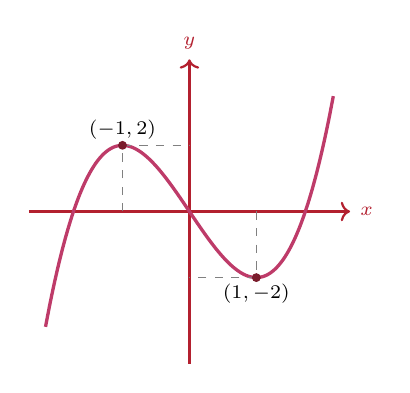
\begin{tikzpicture}[x=0.85cm,y=0.42cm]
\draw[->,thick,redx] (-2.4,0)--(2.4,0) node[right,font=\scriptsize]{$x$};
\draw[->,thick,redx] (0,-4.6)--(0,4.6) node[above,font=\scriptsize]{$y$};
\draw[pinkx!85!black,very thick] plot[domain=-2.15:2.15,samples=70,smooth] (\x,{\x^3-3*\x});
\draw[gray,dashed] (-1,0)--(-1,2)--(0,2) (1,0)--(1,-2)--(0,-2);
\fill[maroon] (-1,2) circle (1.6pt) (1,-2) circle (1.6pt);
\node[font=\scriptsize,above,inner sep=2pt] at (-1,2) {$(-1,2)$};
\node[font=\scriptsize,below,inner sep=2pt] at (1,-2) {$(1,-2)$};
\end{tikzpicture}}}{\pil{$0$}{$1$}{$2$}{$3$}{$5$}}

% =====================================================================
\bagian{B. Isian Singkat}{5 soal $\times$ 4 poin = 20 poin. Tuliskan hanya jawaban akhir.}

\tingkat{Tingkat Sedang}{soal 1 dan 2}
\soal{\gbr{Gambar menunjukkan grafik polinomial $P(x)=x^3+ax^2+bx+c$. Grafik memotong sumbu-$x$ di $x=-3$, menyinggung sumbu-$x$ di $x=1$, dan memotong sumbu-$y$ di $(0,3)$. Nilai $a\cdot b\cdot c$ adalah \dots.}{%
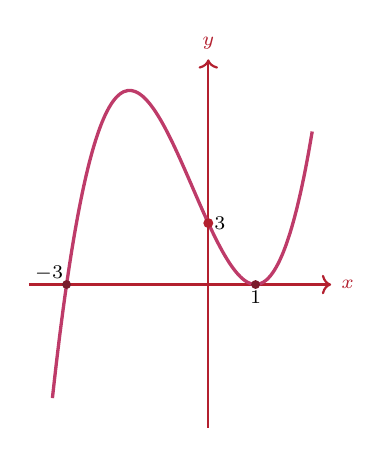
\begin{tikzpicture}[x=0.6cm,y=0.26cm]
\draw[->,thick,redx] (-3.8,0)--(2.6,0) node[right,font=\scriptsize]{$x$};
\draw[->,thick,redx] (0,-7)--(0,11) node[above,font=\scriptsize]{$y$};
\draw[pinkx!85!black,very thick] plot[domain=-3.3:2.2,samples=70,smooth] (\x,{(\x-1)^2*(\x+3)});
\fill[maroon] (-3,0) circle (1.6pt) (1,0) circle (1.6pt);
\fill[redx] (0,3) circle (1.8pt);
\node[font=\scriptsize,above left,inner sep=1pt] at (-3,0) {$-3$};
\node[font=\scriptsize,below,inner sep=2pt] at (1,0) {$1$};
\node[font=\scriptsize,right,inner sep=2pt] at (0,3) {$3$};
\end{tikzpicture}}}{\jwb}
\soal{\gbr{Sebuah balok berukuran panjang $(x+4)$ cm, lebar $x$ cm, dan tinggi $(x-1)$ cm memiliki volume $96$ cm$^3$. Luas permukaan balok tersebut adalah \dots\ cm$^2$.}{%
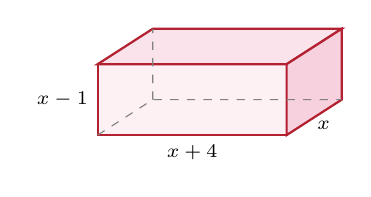
\begin{tikzpicture}
\def\p{2.4}\def\t{0.9}
\coordinate (A) at (0,0); \coordinate (B) at (\p,0); \coordinate (C) at (\p,\t); \coordinate (D) at (0,\t);
\coordinate (dep) at (0.7,0.45);
\draw[redx,thick,fill=softbg] (A)--(B)--(C)--(D)--cycle;
\draw[redx,thick,fill=pinkx!15] (D)--($(D)+(dep)$)--($(C)+(dep)$)--(C)--cycle;
\draw[redx,thick,fill=pinkx!25] (B)--($(B)+(dep)$)--($(C)+(dep)$)--(C)--cycle;
\draw[gray,dashed] (A)--($(A)+(dep)$)--($(B)+(dep)$) ($(A)+(dep)$)--($(D)+(dep)$);
\node[font=\scriptsize,below] at ({\p/2},0) {$x+4$};
\node[font=\scriptsize,left] at (0,{\t/2}) {$x-1$};
\node[font=\scriptsize,below right,inner sep=1pt] at ($(B)+0.5*(dep)$) {$x$};
\end{tikzpicture}}}{\jwb}

\tingkat{Tingkat Sulit}{soal 3 sampai 5}
\soal{Jika $a,b,c$ adalah akar-akar persamaan $x^3-3x^2+5x-4=0$, nilai $(a+b)(b+c)(c+a)$ adalah \dots.}{\jwb}
\soal{Hasil kali semua akar real persamaan $(x^2-3x)^2-2(x^2-3x)-8=0$ adalah \dots.}{\jwb}
\soal{Banyak bilangan bulat $n$ sehingga $\dis\frac{n^3+2n^2-5}{n+3}$ juga bilangan bulat adalah \dots.}{\jwb}

% =====================================================================
\Needspace{16\baselineskip}
\bagian{C. Uraian (Essay)}{5 soal $\times$ 8 poin = 40 poin. Tuliskan langkah penyelesaian dengan lengkap.}

\tingkat{Tingkat Sedang}{soal 1 dan 2}
\soal{Diketahui polinomial $P(x)=2x^3+ax^2-13x+b$. Polinomial ini habis dibagi $x-2$ dan bersisa $18$ jika dibagi $x+1$.\par\smallskip
(a) Tentukan nilai $a$ dan $b$.\par
(b) Faktorkan $P(x)$ sepenuhnya dengan skema Horner.\par
(c) Tentukan semua akar persamaan $P(x)=0$.\par
(d) Tentukan himpunan penyelesaian $P(x)\le0$.}{\poin{8}}
\soal{Diketahui $P(x)=3x^4-2x^3+5x-7$.\par\smallskip
(a) Tentukan hasil bagi dan sisa pembagian $P(x)$ oleh $x^2+x-2$ dengan pembagian bersusun.\par
(b) Periksa kebenaran sisa pada (a) dengan teorema sisa (pakai pembagi $x-1$ dan $x+2$).\par
(c) Tentukan hasil bagi dan sisa jika $P(x)$ dibagi $2x^2+2x-4$.\par
(d) Tentukan polinomial $T(x)$ berderajat paling tinggi $1$ sehingga $P(x)+T(x)$ habis dibagi $x^2+x-2$.}{\poin{8}}

\tingkat{Tingkat Sulit}{soal 3 dan 4}
\soal{\gbr{Sebuah balok memiliki jumlah panjang seluruh rusuk $36$ cm, luas permukaan $52$ cm$^2$, dan volume $24$ cm$^3$. Misalkan panjang, lebar, dan tinggi balok adalah $p$, $l$, dan $t$.\par\smallskip
(a) Tunjukkan bahwa $p$, $l$, dan $t$ adalah akar-akar persamaan $x^3-9x^2+26x-24=0$.\par
(b) Tentukan ukuran balok tersebut.\par
(c) Tentukan panjang diagonal ruang balok.\par
(d) Jika setiap rusuk ditambah $1$ cm, tunjukkan bahwa volume baru adalah $60$ cm$^3$ tanpa mencari akarnya terlebih dahulu.}{%
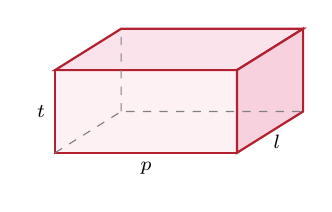
\begin{tikzpicture}[scale=1.05]
\def\p{2.2}\def\t{1.0}
\coordinate (A) at (0,0); \coordinate (B) at (\p,0); \coordinate (C) at (\p,\t); \coordinate (D) at (0,\t);
\coordinate (dep) at (0.8,0.5);
\draw[redx,thick,fill=softbg] (A)--(B)--(C)--(D)--cycle;
\draw[redx,thick,fill=pinkx!15] (D)--($(D)+(dep)$)--($(C)+(dep)$)--(C)--cycle;
\draw[redx,thick,fill=pinkx!25] (B)--($(B)+(dep)$)--($(C)+(dep)$)--(C)--cycle;
\draw[gray,dashed] (A)--($(A)+(dep)$)--($(B)+(dep)$) ($(A)+(dep)$)--($(D)+(dep)$);
\node[font=\scriptsize,below] at ({\p/2},0) {$p$};
\node[font=\scriptsize,left] at (0,{\t/2}) {$t$};
\node[font=\scriptsize,below right,inner sep=1pt] at ($(B)+0.5*(dep)$) {$l$};
\end{tikzpicture}}}{\poin{8}}
\soal{\gbr{Diketahui polinomial $P(x)=2x^4-3x^3-x^2-3x+2$ (grafik pada gambar).\par\smallskip
(a) Tunjukkan bahwa $x=0$ bukan akar, lalu dengan membagi $P(x)=0$ oleh $x^2$ dan memisalkan $t=x+\dfrac1x$, tunjukkan bahwa $2t^2-3t-5=0$.\par
(b) Tentukan semua nilai $t$.\par
(c) Tentukan semua akar real $P(x)=0$.\par
(d) Faktorkan $P(x)$, lalu tentukan himpunan penyelesaian $P(x)<0$.}{%
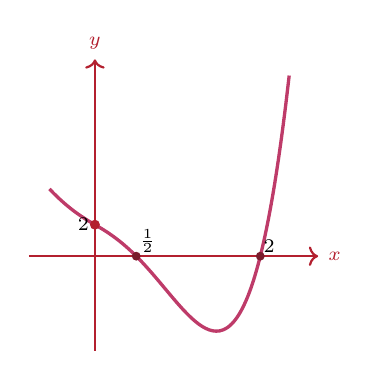
\begin{tikzpicture}[x=1.05cm,y=0.2cm]
\draw[->,thick,redx] (-0.8,0)--(2.7,0) node[right,font=\scriptsize]{$x$};
\draw[->,thick,redx] (0,-6)--(0,12.5) node[above,font=\scriptsize]{$y$};
\draw[pinkx!85!black,very thick] plot[domain=-0.55:2.35,samples=70,smooth] (\x,{2*\x^4-3*\x^3-\x^2-3*\x+2});
\fill[maroon] (0.5,0) circle (1.6pt) (2,0) circle (1.6pt);
\fill[redx] (0,2) circle (1.8pt);
\node[font=\scriptsize,above right,inner sep=1pt] at (0.5,0) {$\frac12$};
\node[font=\scriptsize,above right,inner sep=1pt] at (2,0) {$2$};
\node[font=\scriptsize,left,inner sep=2pt] at (0,2) {$2$};
\end{tikzpicture}}}{\poin{8}}

\tingkat{Tingkat HOTS}{soal 5}
\soal{Polinomial $P(x)=c_nx^n+\cdots+c_1x+c_0$ berkoefisien bulat dan memenuhi $P(1)$ dan $P(2)$ keduanya bilangan ganjil. Kita ingin membuktikan bahwa persamaan $P(x)=0$ tidak mempunyai akar bilangan bulat.\par\smallskip
(a) Untuk bilangan bulat $a\neq b$, buktikan bahwa $(a-b)\mid\big(P(a)-P(b)\big)$. (Petunjuk: $a^k-b^k=(a-b)(a^{k-1}+a^{k-2}b+\cdots+b^{k-1})$.)\par
(b) Buktikan bahwa $P(0)$ ganjil.\par
(c) Misalkan $k$ bilangan bulat dengan $P(k)=0$. Tinjau kasus $k$ genap dan $k$ ganjil, lalu simpulkan bahwa pengandaian tersebut salah.\par
(d) Apakah kebalikannya benar, yaitu jika $P(x)=0$ tidak punya akar bulat maka $P(1)$ dan $P(2)$ ganjil? Berikan contoh penyangkal.}{\poin{8}}

% =====================================================================
\newpage
\bagian{Kunci Jawaban dan Pembahasan Singkat}{Untuk guru dan pembahasan mandiri}
\par\vspace{0.6em}{\bfseries\color{redx}Kunci Pilihan Ganda}\par\vspace{0.3em}
\small
\begin{tabularx}{\linewidth}{@{}*{10}{>{\centering\arraybackslash}X}@{}}\hline \textbf{1} & \textbf{2} & \textbf{3} & \textbf{4} & \textbf{5} & \textbf{6} & \textbf{7} & \textbf{8} & \textbf{9} & \textbf{10}\\ \hline C & E & B & D & A & D & A & E & B & C\\ \hline\end{tabularx}\\[6pt]
\begin{tabularx}{\linewidth}{@{}*{10}{>{\centering\arraybackslash}X}@{}}\hline \textbf{11} & \textbf{12} & \textbf{13} & \textbf{14} & \textbf{15} & \textbf{16} & \textbf{17} & \textbf{18} & \textbf{19} & \textbf{20}\\ \hline B & E & D & A & C & E & C & B & A & D\\ \hline\end{tabularx}
\par\vspace{0.8em}{\bfseries\color{redx}\normalsize Pembahasan Pilihan Ganda}\par\vspace{0.2em}
\small\begin{enumerate}[leftmargin=2em,itemsep=2pt,topsep=2pt]
\item[\textbf{1.}] \textbf{(C)} Derajat $=3+2+1=6$. Koefisien utama $=2^3\cdot1\cdot1=8$. Jumlah $=6+8=14$. (Jebakan: lupa memangkatkan $2$, sehingga memperoleh $6+2=8$.)
\item[\textbf{2.}] \textbf{(E)} Kesamaan berlaku untuk setiap $x$, sehingga substitusi $x=2$ membuat $(x-1)=1$: ruas kanan menjadi $a+b+c$ dan ruas kiri $3(4)-5(2)+7=9$. Jadi $a+b+c=9$. (Cek: $a=3$, $b=1$, $c=5$. Jebakan $5$: menjumlahkan koefisien ruas kiri.)
\item[\textbf{3.}] \textbf{(B)} $P(1)=1+a-5+6=a+2=4\Rightarrow a=2$. Sisa oleh $x+2$ adalah $P(-2)=-8+8+10+6=16$. (Jebakan $12$: memakai $x=2$, padahal pembagi $x+2$ berarti $x=-2$.)
\item[\textbf{4.}] \textbf{(D)} Bentuk faktor: $P(x)=a(x+2)(x-1)(x-3)$. Dari $P(0)=a\cdot2\cdot(-1)\cdot(-3)=6a=12$ diperoleh $a=2$. Maka $P(4)=2\cdot6\cdot3\cdot1=36$. (Jebakan $18$: memakai $a=1$.)
\item[\textbf{5.}] \textbf{(A)} Horner dengan $k=\frac12$ pada koefisien $2,-5,-4,3$ memberi baris hasil $2,-4,-6,0$, sehingga hasil bagi sementara $2x^2-4x-6$ dan sisa $0$. Karena pembagi $2x-1=2\left(x-\frac12\right)$, hasil bagi dibagi $2$: $x^2-2x-3$. (Jebakan B: lupa membagi dengan $2$.) Cek: $(2x-1)(x^2-2x-3)=2x^3-5x^2-4x+3$.
\item[\textbf{6.}] \textbf{(D)} Dari $x^2-4=(x-2)(x+2)$: $P(2)=3(2)+1=7$ dan $P(-2)=-5$. Diketahui juga $P(3)=4$. Sisa oleh $(x-2)(x-3)$ berbentuk $px+q$ dengan $2p+q=7$ dan $3p+q=4$, sehingga $p=-3$ dan $q=13$. Sisa $=-3x+13$. (Jebakan: sisa $3x+1$ adalah sisa oleh $x^2-4$, bukan oleh $(x-2)(x-3)$.)
\item[\textbf{7.}] \textbf{(A)} $P(x)=(x-1)(x-4)(x+2)$ dengan akar $1,4,-2$. (1) \emph{Benar}: $P(-2)=0$. (2) \emph{Benar}: dengan Vieta, $\sum\alpha^2=3^2-2(-6)=21$ (cek: $1+16+4=21$). (3) \emph{Salah}: $P(2)=8-12-12+8=-8$, bukan $8$. (4) \emph{Salah}: $\dis\sum\frac1\alpha=\frac{\sum\alpha\beta}{\alpha\beta\gamma}=\frac{-6}{-8}=\frac34$, bukan $-\frac34$ (jebakan tanda). Cek langsung: $1+\frac14-\frac12=\frac34$.
\item[\textbf{8.}] \textbf{(E)} Calon akar rasional memuat $\pm1,\pm2,\pm3,\pm6,\pm\frac12,\pm\frac32$. $P(2)=16-36+14+6=0$. Horner $k=2$: koefisien $2,-9,7,6$ memberi $2,-5,-3,0$, sehingga $2x^2-5x-3=(2x+1)(x-3)$. Akar-akarnya $2$, $3$, dan $-\frac12$. Selisih terbesar dan terkecil: $3-\left(-\frac12\right)=\frac72$. (Jebakan $\frac52$: $3-\frac12$.)
\item[\textbf{9.}] \textbf{(B)} $P(1)=0\Rightarrow a+b=-6$. $P(-3)=0\Rightarrow81-27a-63-3b+12=0\Rightarrow9a+b=10$. Selisih kedua persamaan: $8a=16$, jadi $a=2$ dan $b=-8$. Nilai $a\cdot b=-16$. (Jebakan: $-6$ adalah $a+b$ dan $10$ adalah $a-b$.) Cek: $P(x)=(x-1)(x+3)(x-2)(x+2)$.
\item[\textbf{10.}] \textbf{(C)} Volume $=x(30-2x)(18-2x)=4x(15-x)(9-x)=448\Rightarrow x^3-24x^2+135x-112=0$. $x=1$ memenuhi. Horner $k=1$: $1,-23,112,0$, sehingga $x^2-23x+112=(x-7)(x-16)$. Akar-akar: $1$, $7$, $16$. Lebar karton $18$ cm sehingga $2x<18$, yaitu $x<9$: $x=16$ ditolak. Jumlah $=1+7=8$. (Jebakan $24$: jumlah semua akar; $23$: jumlah dua akar kuadratnya.)
\item[\textbf{11.}] \textbf{(B)} Karena $x^3-1=(x-1)(x^2+x+1)$, maka $x^3\equiv1$ modulo $x^2+x+1$. $x^{100}=x^{99}\cdot x\equiv x$ dan $x^{50}=x^{48}\cdot x^2\equiv x^2\equiv-x-1$. Sisa $=x+2(-x-1)+3=-x+1$.
\item[\textbf{12.}] \textbf{(E)} $P(x)=a(x+2)(x-1)^2(x-3)$ (akar ganda di $x=1$ karena menyinggung). $P(0)=a\cdot2\cdot1\cdot(-3)=-6a=6\Rightarrow a=-1$. Maka $P(2)=-(4)(1)(-1)=4$ dan $P(-1)=-(1)(4)(-4)=16$. Sisa $px+q$: $2p+q=4$ dan $-p+q=16$, sehingga $p=-4$ dan $q=12$. Sisa $=-4x+12$.
\item[\textbf{13.}] \textbf{(D)} Misalkan akar-akarnya $\frac ar,a,ar$. Hasil kali $a^3=64\Rightarrow a=4$. Jumlah: $4\left(\frac1r+1+r\right)=14\Rightarrow r+\frac1r=\frac52\Rightarrow r=2$ (atau $\frac12$). Akar-akarnya $2,4,8$ dan $k=2\cdot4+2\cdot8+4\cdot8=56$. (Jebakan $64$: hasil kali akar.)
\item[\textbf{14.}] \textbf{(A)} Horner dua kali dengan $k=1$. Pertama, koefisien $1,0,-2,0,0,7$ memberi $1,1,-1,-1,-1,6$: sisa $6$, hasil bagi $x^4+x^3-x^2-x-1$. Kedua, koefisien $1,1,-1,-1,-1$ memberi $1,2,1,0,-1$: sisa $-1$. Jadi $P(x)=(x-1)^2Q_2(x)-(x-1)+6$, sehingga sisa oleh $(x-1)^2$ adalah $-(x-1)+6=-x+7$. (Cek: $P(1)=6=-1+7$.)
\item[\textbf{15.}] \textbf{(C)} $x^4-2x^3-3x^2+4x+4=(x^2-x-2)^2=(x-2)^2(x+1)^2\ge0$ untuk semua $x$. Nilai $\le0$ hanya terjadi saat bernilai nol, yaitu $x=2$ atau $x=-1$. Banyaknya $=2$. (Jebakan $4$: mengira himpunan penyelesaiannya interval $[-1,2]$ sehingga memuat $-1,0,1,2$.)
\item[\textbf{16.}] \textbf{(E)} $Q(x)=P(x)-10x$ berderajat $4$, monik, dan mempunyai akar $1,2,3$, sehingga $Q(x)=(x-1)(x-2)(x-3)(x-r)$. $P(0)=Q(0)=6r$ dan $P(4)=40+Q(4)=40+6(4-r)=64-6r$. Jumlahnya $64$, tidak bergantung pada $r$.
\item[\textbf{17.}] \textbf{(C)} Jumlahkan $P(x+1)-P(x)$ untuk $x=0,1,\dots,5$ (teleskopik): $P(6)-P(0)=\sum_{x=0}^{5}(6x^2+4x+1)=6(55)+4(15)+6=396$. Jadi $P(6)=4+396=400$. (Jebakan $396$: lupa menambahkan $P(0)$.) Cek: $P(x)=2x^3-x^2+4$.
\item[\textbf{18.}] \textbf{(B)} (1) \emph{Benar}: akar tak real muncul berpasangan (konjugat), jadi akar kubik pasti memuat akar real. (2) \emph{Salah}: $x^4+4=(x^2+2)^2-(2x)^2=(x^2+2x+2)(x^2-2x+2)$. (3) \emph{Benar}: $p+q=2$ dan $-p+q=2$ memberi $p=0$ dan $q=2$. (4) \emph{Salah}: untuk $P(x)=x$, $P(7)-P(3)=4$ tidak habis dibagi $5$; yang pasti terpenuhi adalah habis dibagi $7-3=4$. Urutan: B, S, B, S.
\item[\textbf{19.}] \textbf{(A)} Vieta: $\sum a=2$, $\sum ab=3$, $abc=5$. Untuk akar kuadrat: $\sum a^2=2^2-2(3)=-2$; $\sum a^2b^2=(\sum ab)^2-2abc\sum a=9-20=-11$; $a^2b^2c^2=25$. Persamaan: $y^3-(-2)y^2+(-11)y-25=0$, yaitu $x^3+2x^2-11x-25=0$. (Jebakan D: mengkuadratkan koefisien secara langsung.)
\item[\textbf{20.}] \textbf{(D)} Persamaan $x^3-3x=k$ berarti garis mendatar $y=k$ memotong grafik. Tiga titik potong berbeda terjadi jika $-2<k<2$, yaitu $k=-1,0,1$. Untuk $k=\pm2$ garis menyinggung di satu titik balik sehingga hanya ada dua akar berbeda. Banyaknya $=3$. (Jebakan $5$: ikut menghitung $k=\pm2$.)
\end{enumerate}
\par\Needspace{6\baselineskip}\vspace{0.6em}{\bfseries\color{redx}\normalsize Pembahasan Isian Singkat}\par\vspace{0.2em}
\small\begin{enumerate}[leftmargin=2em,itemsep=2pt,topsep=2pt]
\item[\textbf{1.}] \textbf{Jawaban: $-15$.} Koefisien $x^3$ adalah $1$, akar tunggal $-3$ dan akar ganda $1$: $P(x)=(x-1)^2(x+3)=x^3+x^2-5x+3$. Titik $(0,3)$ sesuai. Jadi $a=1$, $b=-5$, $c=3$ dan $abc=-15$.
\item[\textbf{2.}] \textbf{Jawaban: $136$.} Volume: $x(x+4)(x-1)=96\Rightarrow x^3+3x^2-4x-96=0$. $x=4$ memenuhi; Horner $k=4$: $1,7,24,0$ dan $x^2+7x+24$ tidak punya akar real (diskriminan $49-96<0$). Ukuran balok $8\times4\times3$. Luas permukaan $=2(8\cdot4+8\cdot3+4\cdot3)=2(68)=136$ cm$^2$.
\item[\textbf{3.}] \textbf{Jawaban: $11$.} Karena $a+b+c=3$, maka $a+b=3-c$ dan seterusnya, sehingga $(a+b)(b+c)(c+a)=(3-a)(3-b)(3-c)=P(3)$ dengan $P(x)=x^3-3x^2+5x-4$. Jadi hasilnya $27-27+15-4=11$.
\item[\textbf{4.}] \textbf{Jawaban: $-8$.} Misalkan $u=x^2-3x$: $u^2-2u-8=0\Rightarrow(u-4)(u+2)=0$. Untuk $u=4$: $x^2-3x-4=0$ memberi $x=4,-1$. Untuk $u=-2$: $x^2-3x+2=0$ memberi $x=1,2$. Hasil kali $=4\cdot(-1)\cdot1\cdot2=-8$.
\item[\textbf{5.}] \textbf{Jawaban: $8$.} $n^3+2n^2-5=(n+3)(n^2-n+3)-14$, sehingga pecahan bulat jika dan hanya jika $(n+3)\mid14$. Nilai $n+3\in\{\pm1,\pm2,\pm7,\pm14\}$, yaitu $8$ nilai $n$ (yaitu $-17,-10,-5,-4,-2,-1,4,11$).
\end{enumerate}
\par\Needspace{8\baselineskip}\vspace{0.6em}{\bfseries\color{redx}\normalsize Pembahasan dan Pedoman Penskoran Uraian}\par\vspace{0.2em}
\small\begin{enumerate}[leftmargin=2em,itemsep=3pt,topsep=2pt]
\item[\textbf{1.}] (a) $P(2)=16+4a-26+b=0\Rightarrow4a+b=10$. $P(-1)=-2+a+13+b=18\Rightarrow a+b=7$. Maka $a=1$ dan $b=6$, sehingga $P(x)=2x^3+x^2-13x+6$. (b) Horner $k=2$: koefisien $2,1,-13,6$ memberi $2,5,-3,0$. Hasil bagi $2x^2+5x-3=(2x-1)(x+3)$, sehingga $P(x)=(x-2)(2x-1)(x+3)$. (c) Akar-akar: $x=2$, $x=\frac12$, dan $x=-3$. (d) Koefisien utama positif sehingga grafik naik di kanan. Tanda $P$ dari kanan ke kiri: positif untuk $x>2$, negatif pada $\frac12<x<2$, positif pada $-3<x<\frac12$, negatif untuk $x<-3$. Jadi $P(x)\le0$ untuk $x\le-3$ atau $\frac12\le x\le2$. \\ \textit{Penskoran: (a) 2 poin; (b) 2 poin; (c) 2 poin; (d) 2 poin.}
\item[\textbf{2.}] (a) Pembagian bersusun: $3x^4-2x^3+5x-7-3x^2(x^2+x-2)=-5x^3+6x^2+5x-7$; lalu $-5x(x^2+x-2)$ menyisakan $11x^2-5x-7$; lalu $11(x^2+x-2)$ menyisakan $-16x+15$. Hasil bagi $3x^2-5x+11$ dan sisa $-16x+15$. (b) $P(x)=(x-1)(x+2)H(x)+S(x)$ sehingga $P(1)=S(1)$ dan $P(-2)=S(-2)$. $P(1)=3-2+5-7=-1$ dan $S(1)=-16+15=-1$. $P(-2)=48+16-10-7=47$ dan $S(-2)=32+15=47$. Sesuai. (c) $2x^2+2x-4=2(x^2+x-2)$, sehingga hasil bagi dibagi $2$: $\frac32x^2-\frac52x+\frac{11}2$, sedangkan sisanya tetap $-16x+15$ (sisa tidak berubah). (d) $P(x)+T(x)=(x^2+x-2)H(x)+\big(S(x)+T(x)\big)$, habis dibagi jika $T(x)=-S(x)=16x-15$. \\ \textit{Penskoran: (a) 2 poin; (b) 2 poin; (c) 2 poin; (d) 2 poin.}
\item[\textbf{3.}] (a) $4(p+l+t)=36\Rightarrow p+l+t=9$. $2(pl+lt+tp)=52\Rightarrow pl+lt+tp=26$. $plt=24$. Polinomial yang akar-akarnya $p,l,t$ adalah $x^3-(p+l+t)x^2+(pl+lt+tp)x-plt=x^3-9x^2+26x-24$. (b) $x=2$ akar: $8-36+52-24=0$. Horner $k=2$: $1,-7,12,0$ dan $x^2-7x+12=(x-3)(x-4)$. Ukuran balok $2\times3\times4$ cm. (c) $d=\sqrt{p^2+l^2+t^2}=\sqrt{(p+l+t)^2-2(pl+lt+tp)}=\sqrt{81-52}=\sqrt{29}$ cm (cek: $4+9+16=29$). (d) $(p+1)(l+1)(t+1)=plt+(pl+lt+tp)+(p+l+t)+1=24+26+9+1=60$ cm$^3$. Cara lain: bila $P(x)=x^3-9x^2+26x-24$, maka $(p+1)(l+1)(t+1)=-P(-1)=1+9+26+24=60$. \\ \textit{Penskoran: (a) 2 poin; (b) 2 poin; (c) 2 poin; (d) 2 poin.}
\item[\textbf{4.}] (a) $P(0)=2\neq0$, jadi $x\neq0$ dan $P(x)=0$ boleh dibagi $x^2$: $2x^2-3x-1-\frac3x+\frac2{x^2}=0$, yaitu $2\left(x^2+\frac1{x^2}\right)-3\left(x+\frac1x\right)-1=0$. Karena $x^2+\frac1{x^2}=t^2-2$, diperoleh $2(t^2-2)-3t-1=0\Rightarrow2t^2-3t-5=0$. (b) $(2t-5)(t+1)=0\Rightarrow t=\frac52$ atau $t=-1$. (c) $t=\frac52$: $x+\frac1x=\frac52\Rightarrow2x^2-5x+2=0\Rightarrow x=2$ atau $x=\frac12$. $t=-1$: $x^2+x+1=0$ dengan diskriminan $-3<0$ (tidak ada akar real). Akar real: $x=2$ dan $x=\frac12$. (d) $P(x)=(x-2)(2x-1)(x^2+x+1)$. Karena $x^2+x+1>0$ untuk semua $x$ (koefisien utama positif dan diskriminan negatif), $P(x)<0\iff(x-2)(2x-1)<0\iff\frac12<x<2$. Sesuai gambar. \\ \textit{Penskoran: (a) 2 poin; (b) 1 poin; (c) 3 poin (akar $t=\frac52$ 2, penolakan $t=-1$ 1); (d) 2 poin.}
\item[\textbf{5.}] (a) $P(a)-P(b)=\sum_{k}c_k(a^k-b^k)$ dan tiap $a^k-b^k=(a-b)(a^{k-1}+\cdots+b^{k-1})$ merupakan kelipatan $a-b$ (bilangan bulat). Jadi $(a-b)\mid P(a)-P(b)$. (b) Pakai $a=2$, $b=0$: $2\mid P(2)-P(0)$, sehingga $P(2)-P(0)$ genap. Karena $P(2)$ ganjil, $P(0)$ ganjil. (c) Misalkan $k$ bulat dan $P(k)=0$. Kasus $k$ genap: jika $k=0$, maka $P(0)=0$ bertentangan dengan (b). Jika $k\neq0$ genap, $k\mid P(k)-P(0)=-P(0)$, yaitu bilangan ganjil, tetapi bilangan genap tidak dapat membagi bilangan ganjil (kontradiksi). Kasus $k$ ganjil: jika $k=1$, $P(1)=0$ bertentangan dengan $P(1)$ ganjil. Jika $k\neq1$, maka $k-1$ genap dan tidak nol, dan $(k-1)\mid P(k)-P(1)=-P(1)$, yaitu bilangan ganjil (kontradiksi). Jadi tidak ada akar bulat. (d) Tidak. Contoh penyangkal: $P(x)=x^2+1$ tidak punya akar bulat (bahkan tidak punya akar real), tetapi $P(1)=2$ genap. \\ \textit{Penskoran: (a) 2 poin; (b) 2 poin; (c) 3 poin (kasus genap 1,5, kasus ganjil 1,5); (d) 1 poin.}
\end{enumerate}
\end{document}
